\chapter{Features}\label{chap:features}

\section{Notifications and Comments}

The following section describes an important part of the application, especially for registered users: the notification system and the opportunity of adding comments basically to any resource in the system.

\subsection{Activity stream}
It displays the most recent events in the portal in descending order. Each activity (see figure \ref{fig:activity-stream-single-activity}), one line in the stream, consists of 3 parts: meta information about the activity itself, information about the initiator and comments. The content of each of these parts is being determined automatically, when a new notification is being persisted to the database.

Besides the initiator information and comments, each activity has an own title, description and an icon. These meta information texts can be edited in the portal in the 'Administration' > 'Actions' section. A fixed set of notifcations is provided in the portal, they are editable but not removable.

\begin{figure}[!h]
  \centering
  \fbox{
    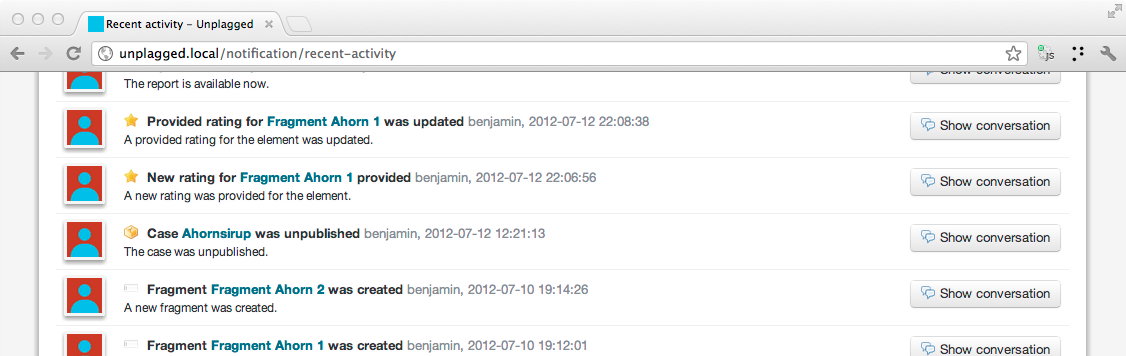
\includegraphics[width=0.97\textwidth]{images/feature-activity-stream.png}
  }
  \caption{Single activity in the activity stream}
  \label{fig:activity-stream-single-activity}
\end{figure}

The following code snippet shows, how to create a new notification when a new automatic plagiarism detection report was created. The static method takes in 3 parameters: a unique name for the notification type, the content object related to the notification and a user object, as the third parameter. A list of all available notification types can either be found in the previousely mentioned actions section or in the scripts/build/initdb.php file, where all notifcation types are being declared.

\begin{lstlisting}[caption=Creating a notification for a created report]
Unplagged_Helper::notify("detection_report_created", $report, $report->getUser());
\end{lstlisting}

Unplagged does have an extensive role and permission management. Therefore the grant on each resource is verified, before it is displayed in the activity stream. Usually the resource related to the notification and the resource the permission check is performed on are the same. Although in some cases, e.g. when rating a fragment, the resource will be the rating itself, but the permission check is done on the fragment. In this case the notify-method is called with a fourth, optional parameter, another resource, in this case the fragment. When the user has access on the fragment, all ratings can be accessed as well, automatically and so are the notifcations.

\subsection{Comments plugin}

Comments are simply a small text related to a specific user and a resource. They can be used to share ideas on a content object collaboratively. The most prominent part at Unplagged, where comments are being used, is the activity stream. A comment can be added by any user having access to the notification. 

\begin{figure}[!h]
  \centering
  \fbox{
    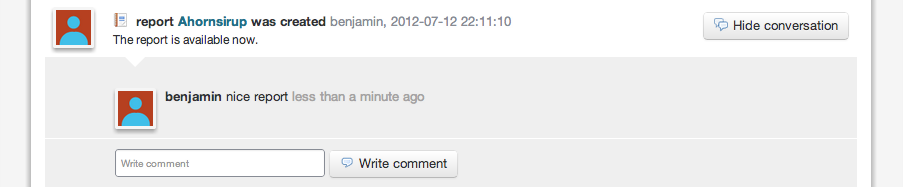
\includegraphics[width=0.97\textwidth]{images/feature-comment.png}
  }
  \caption{Creating a comment on a resource}
  \label{fig:creating-a-comment}
\end{figure}

For providing a better workflow to the user, the comments can be refreshed and added in place. That means, the position where the user scrolled to in the browser does not get affected. The in-place refreshing is realized through AJAX. The comments container is loaded empty and displaying a small loading image only. Not before the user clicks the 'show conversation' button, the comments are being fetched through a post request to the server. Whenever the result is fetched completely, the spinner graphic is hidden and the comments are appended. The parsing of the comments markup is done in Javascript as well. So the server requests are kept small and the server can return JSON only without any HTML.

\begin{lstlisting}[caption=Refreshing the comments of a resource]
	target.show();
      conversation.hide();
      loading.slideDown(800, function() {
        // get the whole conversation
        $.post('/notification/conversation', {
          'source': sourceId
        }, function(data) {
          if(!data.errorcode) {
            conversation.html("");
            $.each(data, function(index, value) {
              conversation.append(renderConversation(value));
            });
            loading.slideUp(800, function() {
              conversation.slideDown(300);
            });
          } else {
            conversation.html('<div class="comment">' + data.message + '</div>');
            loading.slideUp(800, function() {
              conversation.slideDown(300);
            });
          }
        }, "json");
\end{lstlisting}

\begin{lstlisting}[caption=Creating the markup of a single comment]
function renderConversation(data, target) {
    var tpl;
    
    switch(data.type) {
      case 'comment':
        tpl = '<div class="comment">' +
        '<div class="image"><img class="avatar-small" src="' + data.author.avatar + '" /></div>' +
        '<div class="details">' +
        '<div class="title"><b>' + data.author.username + '</b> ' + data.text + 
        ' <span class="date">' + data.created.humanTiming + '</span>' +
        '</div>' +
        '</div>' +
        '</div>';
        break;
    }
    if(!target) {
      return tpl;
    } else {
      target.append(tpl);
    }
  }
\end{lstlisting}

\section{Fragments}

Fragments are the part of the application where found text passages that are plagiairism or potential plagiarism are being documented.

A single fragment contains a candidate and a source document. Each of the two documents is being saved with a starting position (page number / line number combination) and an ending position. These two positions can be used to determine exactly the text being involved in a fragment. To visualize this, the figure \ref{fig:single-fragment}) below shows a sample fragment.

\begin{figure}[!h]
  \centering
  \fbox{
    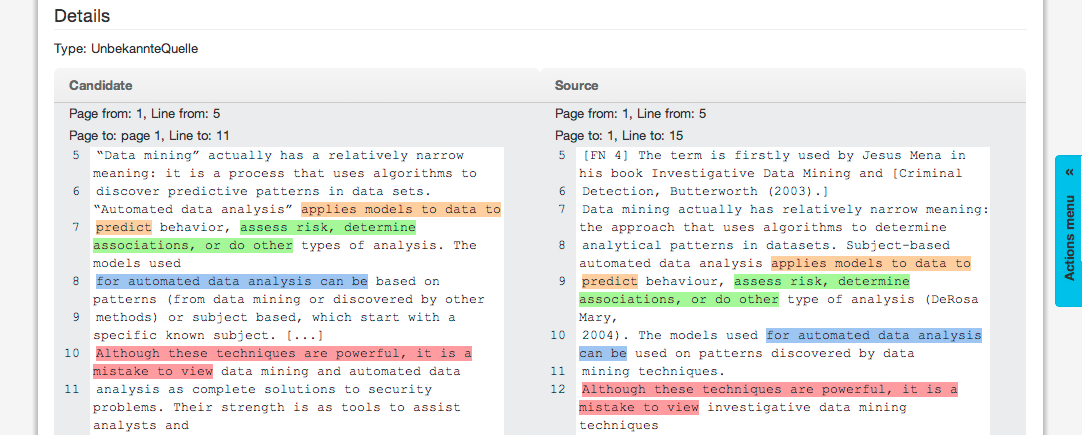
\includegraphics[width=0.97\textwidth]{images/feature-fragment.png}
  }
  \caption{Single fragment with highlighted similarities}
  \label{fig:single-fragment}
\end{figure}

\subsection{Creating a fragment}

Such a fragment can be created in two ways, one for people that like using the mouse and another one that can be used with the keyboard only.

\textbf{The old-fashioned way}

The basic way, which can be accessed through the keyboard only, offers a two-column form to the user where the source and potential plagiarism information can be selected by hand. Once a page or line number is being changed, the text shown below is being updated instantly through AJAX and the similarities are highlighted automatically. Although the big disadvantage of this method is, that the whole page is never displayed and the user actually has to guess where the starting and ending point of the fragment in the text really is. Therefore the values of the line from and line to fields have to be increased or decreased by hand, until they are adjusted properly.

\begin{figure}[!h]
  \centering
  \fbox{
    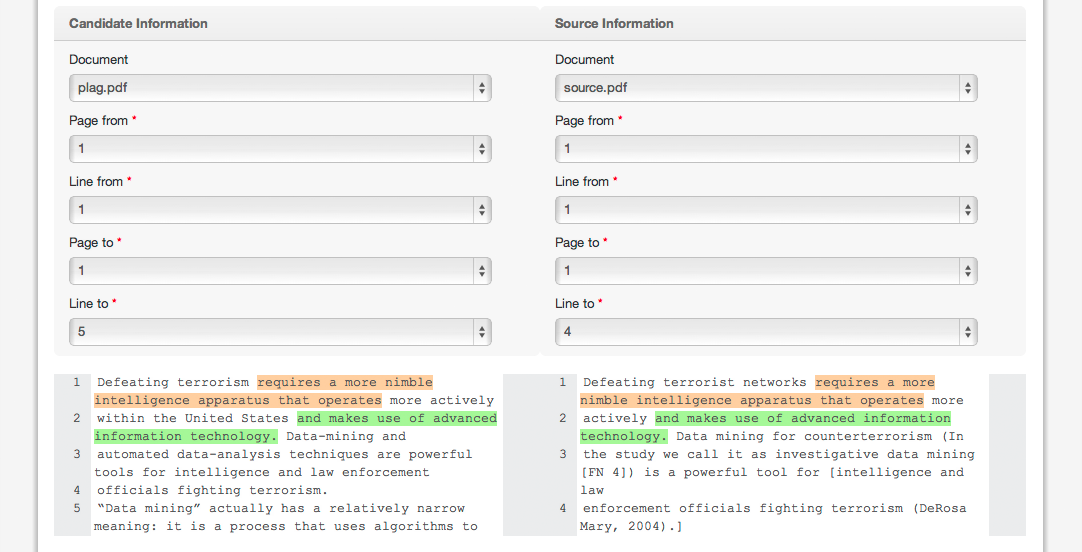
\includegraphics[width=0.97\textwidth]{images/fragment-form.png}
  }
  \caption{Form for creating a fragment by hand}
  \label{fig:fragment-form}
\end{figure}

\textbf{A more comfortable workflow}

Wouldn't it be cool to select text by just marking it with the mouse and having this previousely described form being filled out automatically? We though it would, so we implemented it. 

The user has to go to the document being inspected in the current case, select a page to start with and then hit the button 'Switch to two-column view for fragment creation'. At this point a second document can be selected on the right side and the similarities in both texts are once again being highlighted. (figure \ref{fig:creating-fragment-modern-way-1}) In this two-column view it is also possible to iterate through the pages of the left-side or right-side document to compare page 1 from the left with page 2 from the right and page 1 on the left with page 3 on the right just by one click.

\begin{figure}[!h]
  \centering
  \fbox{
    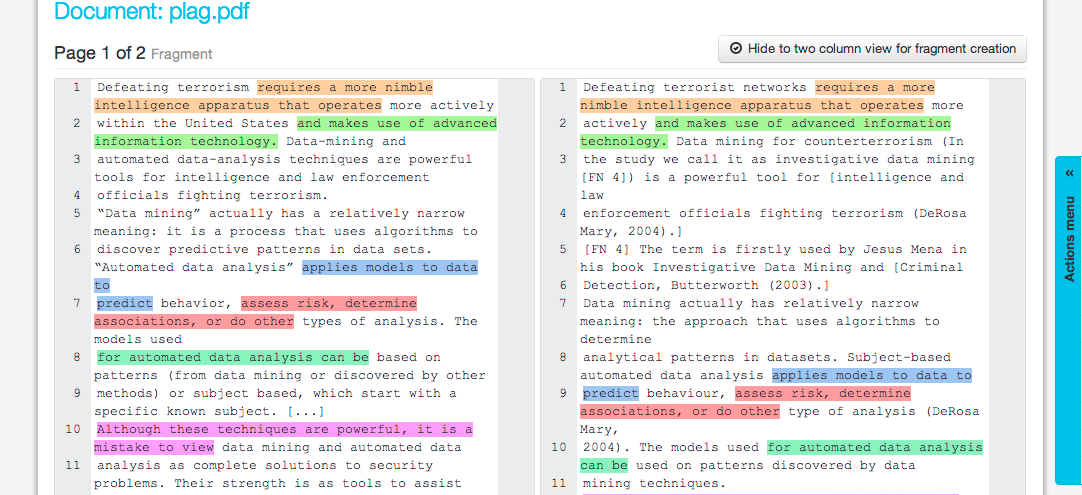
\includegraphics[width=0.97\textwidth]{images/fragment-modern-way-1.png}
  }
  \caption{Creating a fragment the modern way - Step 1}
  \label{fig:creating-fragment-modern-way-1}
\end{figure}

When there are sufficient similarities in an area of the page, a fragment can be created by marking the text, then making a click with the right mouse key to open the context menu and 'set as candidate/source of fragment'. This stores the marked text temporarily until the 'create fragment' button in the context menu is being pressed  (figure \ref{fig:creating-fragment-modern-way-2}). The selection of the 'create fragment' button opens the same form as described in the section before and pre-fills it with the start and end values for page and line for both sides automatically.

This techchnique makes it much easier to create a fragment, since the text can be seen in the context of the whole page, before it is added to the fragment form.

\begin{figure}[!h]
  \centering
  \fbox{
    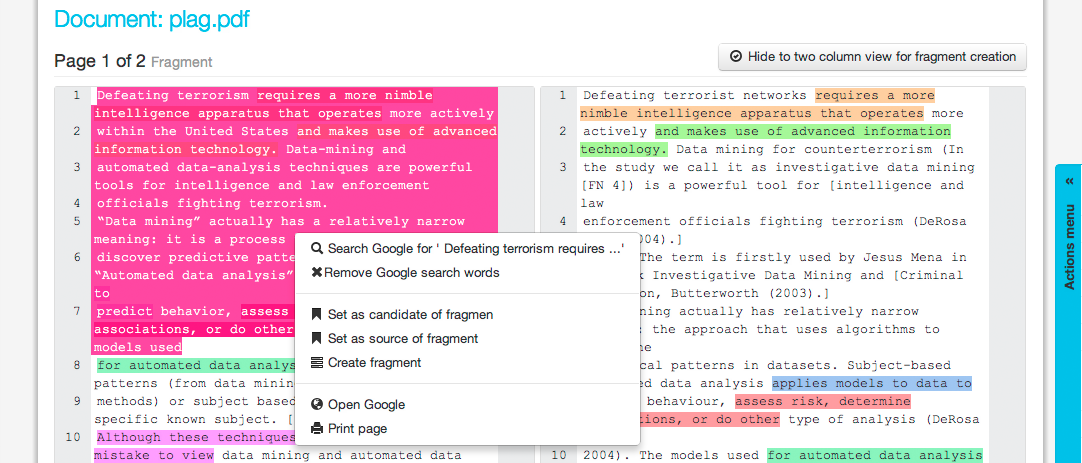
\includegraphics[width=0.97\textwidth]{images/fragment-modern-way-2.png}
  }
  \caption{Creating a fragment the modern way - Step 2}
  \label{fig:creating-fragment-modern-way-2}
\end{figure}

\subsection{Rating a fragment}

A created fragment has to be verified by other collaborators of the case in order to be approved for containing plagiarism. This process is described in the current section.

A rating contains information about the user who made the rating, a flag whether it approves or declines the fragment and an optional property that can contain a description, why the user gave the rating. Each fragment can be approved by a user only once. However the reason and rating type can be changed by the initiator at any time, until the fragment is approved by a certain amount of people. The amount of ratings to lock a fragment and its ratings for further edits is defined in the case administration form. Whenever this amount is reached, the fragment gets locked automatically and can be unlocked by administrators only.

\begin{figure}[!h]
  \centering
  \fbox{
    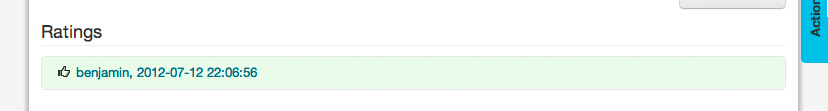
\includegraphics[width=0.97\textwidth]{images/feature-single-rating.png}
  }
  \caption{List of fragment ratings}
  \label{fig:feature-single-rating}
\end{figure}

\section{User avatar}
With the `User avatar' the user gets the possibility to upload a picture to his own profile. Through the function `Profil edititieren'  the user gets to the `Profil editieren' form. 
\pagebreak

\begin{figure}[!h]
  \centering
  \fbox{
    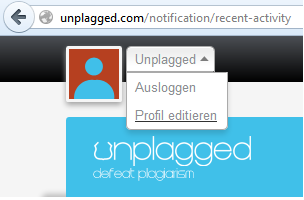
\includegraphics[width=0.97\textwidth]{images/profil_editieren.png}
  }
  \caption{edit profile}
  \label{fig:profil_editieren}
\end{figure}

The uploader in this form allows the user to upload a picture as his avatar.

\pagebreak

\begin{figure}[!h]
  \centering
  \fbox{
    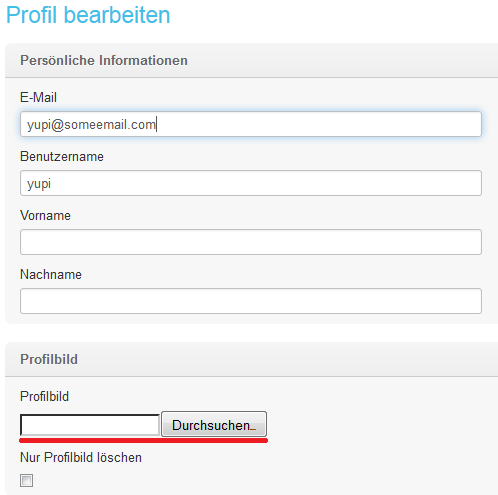
\includegraphics[width=0.97\textwidth]{images/profil_editieren_uploader.png}
  }
  \caption{profile avatar uploader}
  \label{fig:profil_editieren_uploader}
\end{figure}


\subsection{Avatar cropping}

While the previous section described how the user avatar can be set, this one explains how the cropping of images that are not in the correct aspect ratio is done. All avatars have to be in a square aspect ratio. However, not all users have the skills to provide an image that meets these requirements. So we decided to crop uploaded images into the appropriate format after they are uploaded.

What we do is taking the shortest of the two rectangle sides and cut a partial from the center of the longer one of the two sides, which has the same length as the shortest side. To make it more visual what that means, figure \ref{fig:cropping-avatar} shows an example. The red area is the part that will be cropped.

\begin{figure}[!h]
  \centering
  \fbox{
    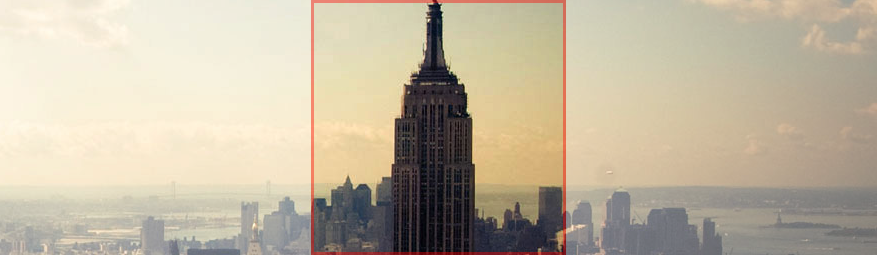
\includegraphics[width=0.97\textwidth]{images/cropped-avatar.png}
  }
  \caption{Cropping avatar}
  \label{fig:cropping-avatar}
\end{figure}

The cropped image then is scaled to the needed width and height, currently 50 x 50 pixels. The algorithm for cropping that has been developed, is shown in the following code snippet.

\begin{lstlisting}[caption=Cropping an image to a square aspect ratio]
public function crop($thumbWidth, $thumbHeight){
    //getting the image dimensions
    list($width, $height) = getimagesize($this->file->getFullPath());
    
    //saving the image into memory (for manipulation with GD Library)
    $myImage = imagecreatefromjpeg($this->file->getFullPath());

    // setting the crop size
    if($width < $height) {
      $twidth = $width;
      $theight = $width;
      $x = 0;
      $y = $height / 2. - $width / 2.;
    } else {
      $twidth = $height;
      $theight = $height;
      $x = $width / 2. - $height / 2.;
      $y = 0;
    }

    // creating the thumbnail
    $thumb = imagecreatetruecolor($thumbWidth, $thumbHeight);
    imagecopyresampled($thumb, $myImage, 0, 0, $x, $y, $thumbWidth, $thumbHeight, $twidth, $theight);

    imagejpeg($thumb, $this->file->getFullPath());

    imagedestroy($thumb);
    imagedestroy($myImage);

    return $this->file;
  }
\end{lstlisting}


\section{Automatic Plagiarism Detection Webservices}

Unplagged itself is a workbench, where the plagiairism detection is done by hand. Although it provides useful automatic tools that help the user to make the process of plagiairism detection easier. One of these tools are external webservices that check a specific text for plagiairism and try to find sources which can be used for further inspections.

We were talking to 3 companies offering such a webservice: Docoloc, PlagScan and PlagAware. As a proof of concept the PlagAware webservice has been implemented and added to our application, it will be described in the following section.

\subsection{PlagAware}

PlagAware, a website for automatic plagairism detection is a commercial website which costs money depending on the amount of text to analyze. It figures out possible sources of the text handed in on their website and creates a PDF report with a list of all the found sources (figure \ref{fig:plagaware-result}).

\begin{figure}[!h]
  \centering
  \fbox{
    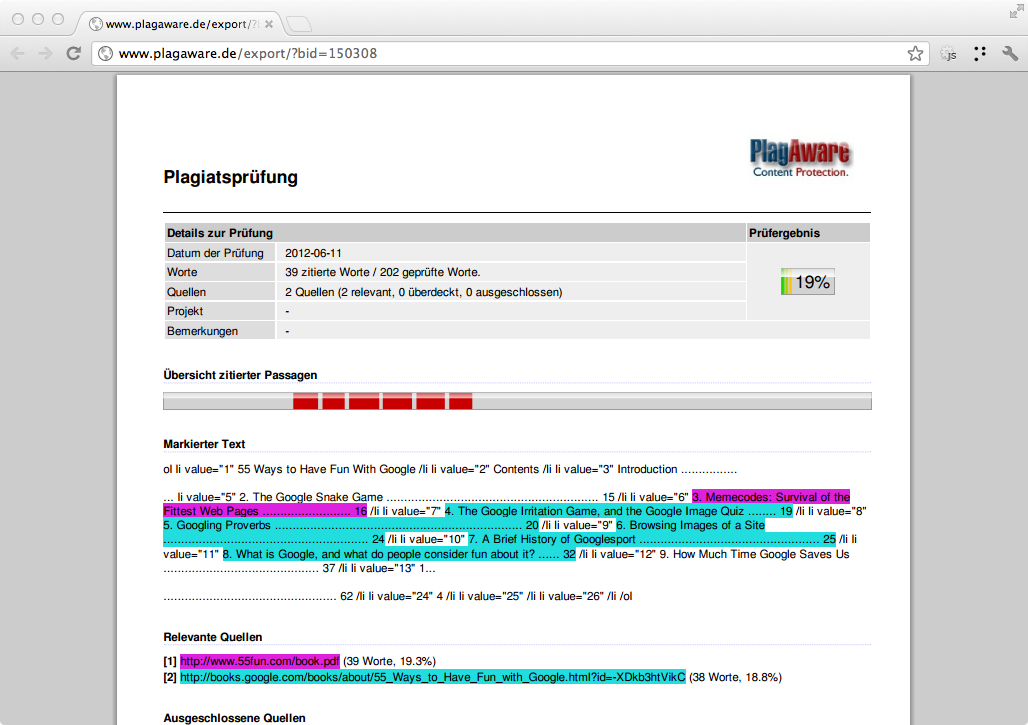
\includegraphics[width=0.97\textwidth]{images/feature-plagaware-result.png}
  }
  \caption{PlagAware result document}
  \label{fig:plagaware-result}
\end{figure}

The website also offers a webservice which takes text as input and notifies the user when the analyzing is finished. Although it does not provide any information about the sources through the webservice response call, there is only a status code and the percentage of plagairism responded. Whenever the response was sent, the user has to go to the PlagAware website and check out the detailed results there.

Since the PlagAware webservice is a simple HTTP-Webservice, the connection is done through an HTTP request with curl.
\begin{lstlisting}[caption=Sending a request through curl to the PlagAware webservice]
public function detect(Application_Model_Document_Page_DetectionReport &$report){
    $url = "http://www.plagaware.de/service/submittext";
    $fields = array(
      'UserCode'=>urlencode($this->paUserCode),
      'ResultUrl'=>urlencode($this->paResultUrl . $report->getId()),
      'TestText'=>urlencode($report->getPage()->getContent()),
      'DryRun'=>urlencode($this->paDryRun)
    );

    // url-ify the data for the POST
    $fields_string = "";
    foreach($fields as $key=>$value){
      $fields_string .= $key . '=' . $value . '&';
    }
    rtrim($fields_string, '&');

    $ch = curl_init();
    curl_setopt($ch, CURLOPT_URL, $url);
    curl_setopt($ch, CURLOPT_RETURNTRANSFER, 1);
    curl_setopt($ch, CURLOPT_CONNECTTIMEOUT, 10);
    curl_setopt($ch, CURLOPT_POST, count($fields));
    curl_setopt($ch, CURLOPT_POSTFIELDS, $fields_string);

    $output = curl_exec($ch);
    $info = curl_getinfo($ch);
    curl_close($ch);
}
\end{lstlisting}

The response is sent through a GET-Request to a pre-defined request URL, in our case '/document/response-plagiarism/report/<report-id>'. The call of this action stores the result in our database and creates a notifcation for the user, indicating that a new report is available.

\section{Permission and role management}

Unplagged does offer an extensive permission and role management, which controls access to pages and entities within the system. It contains two important parts: roles and permissions. A permission is a actually a single right on a resource within the portal and roles are collections of permissions.

\subsection{Roles}

Roles are being used for assigning pre-defined sets of permissions to a single user in different situations. There exist 4 different types of roles, with different characteristics:

\begin{itemize}
\item    	Global roles
\item   	User roles  
\item    	Case default roles
\item   	Case roles
\end{itemize}

Besides the different role types, there exists a concept of role inheritance in our system. One role can inherit from another one, in this case, a user does have the joined rights of the main role and the inherited role as well. 

\textbf{Global roles}

To make this more visual, let's start with the global roles. Global roles include default roles for guests, registered users and admins. A non-registered user does have the guest role by default, a registered user the user role. Since administrative users need some more privilleges, they need the admin role as well. Since the admin role is an inheritable role, it extends the user role and user get's all the rights which are either in the user role or in the admin role.

\textbf{User roles}

When a user registeres on the plattform, a copy of the global user role is created and assigned to the user as it's default role. This role can be modified for each user without influencing other users, so one user can have completely different rights than another one.

\textbf{Case default roles}

All the permissions defined in the roles described above are related to all cases the user is taking part in. Although often it is necessary to add different rights to a user in different cases. For example in one case a user can access all documents, in another one the user can access the files area only. For this case two case default roles are provided: an admin role and a collaborator role, they can be seen as a global role on the case level, used as templates for all cases. 

\textbf{Case roles}

When a new case is created, the same process as described for the user roles takes part, a copy of the case default roles is created, they can be assigned to any collaborator of the case (figure \ref{fig:collaborators-form}). A case role can be added to a user by accessing the Case > Edit form in the 'case collaborators' section. An autocompletion field let's the user search for collaborators by username and then through a dropdown, the role can be selected, as shown in figure \ref{fig:collaborators-form}.

\begin{figure}[!h]
  \centering
  \fbox{
    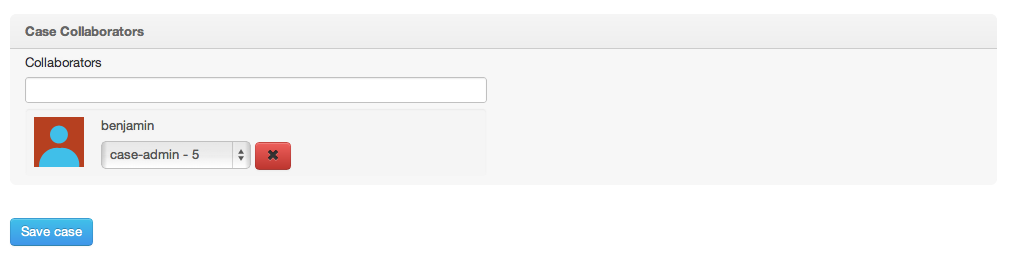
\includegraphics[width=0.97\textwidth]{images/collaborators-form.png}
  }
  \caption{Roles overview}
  \label{fig:collaborators-form}
\end{figure}

All the different roles used in Unplagged can be managed in the Administration > Roles area (figure \ref{fig:roles-list} and figure \ref{fig:roles-form}).

\begin{figure}[!h]
  \centering
  \fbox{
    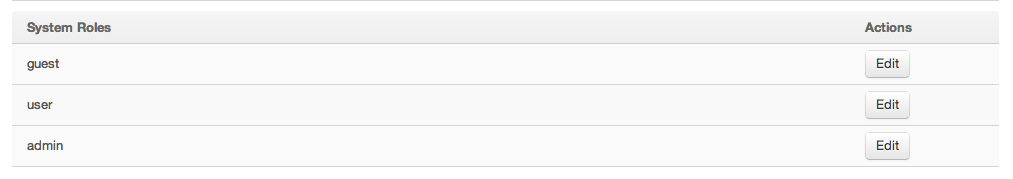
\includegraphics[width=0.97\textwidth]{images/roles-list.png}
  }
  \caption{Roles overview}
  \label{fig:roles-list}
\end{figure}

\begin{figure}[!h]
  \centering
  \fbox{
    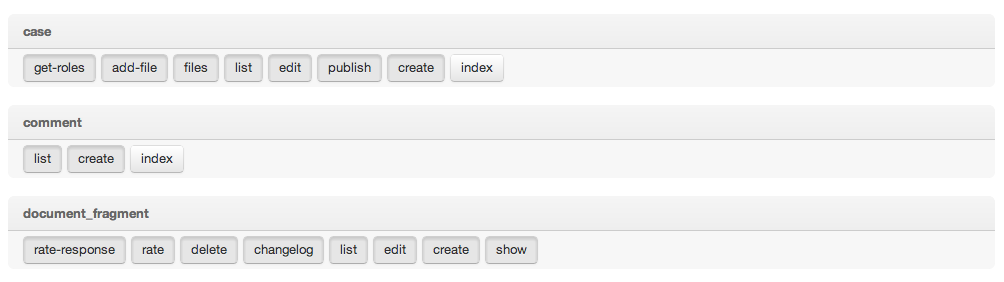
\includegraphics[width=0.97\textwidth]{images/roles-form.png}
  }
  \caption{Role form}
  \label{fig:roles-form}
\end{figure}

\subsection{Permission types}

There exist two permission types which are extending from an abstract permission model – page permissions and model permissions. How they differ from each other will be described further on. Usually a permission is related to a specific object, but we also do have global permissions, which define access to all entities of a kind. 

A single permission basically contains four properties:

\begin{itemize}
\item      type – what model / page type is protected (e.g. document, file, case) 
\item      action – what action of the type (e.g. read, list, create)
\item      base – which entity is protected (e.g. a real entity id or a * for global rights)
\item      permission type – page permission or model permission
\end{itemize}

When a user does not have access to a page resource or a model resource, one is redirected to the previously accessed page automatically.

\textbf{Model permissions}

The ModelPermission entity manages access to single objects within the system, this includes for example cases, files, documents, fragments and comments. Each of them currently has a fixed set of permission actions, based on the CRUD design pattern – create, read, update, delete and a fifth one called authorize. The authorize permission allows a user to control the permissions on a specific entity.

If the user does have the authorize permission on an entity, the form to edit them, can accessed through the actions menu in the list view of the object, as shown in figure \ref{fig:add-model-permission}. 

\begin{figure}[!h]
  \centering
  \fbox{
    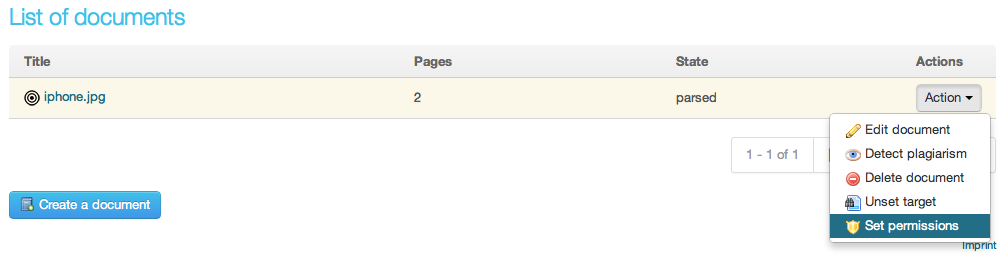
\includegraphics[width=0.97\textwidth]{images/add-model-permission.png}
  }
  \caption{Access form for editing model permissions}
  \label{fig:add-model-permission}
\end{figure}

The form provided to set the permissions offers an autocompletion textfield at the top, where usernames can be searched and afterwards the permissions can be defined by enabling or disabling the buttons below the username (figure \ref{fig:set-model-permissions}).

\begin{figure}[!h]
  \centering
  \fbox{
    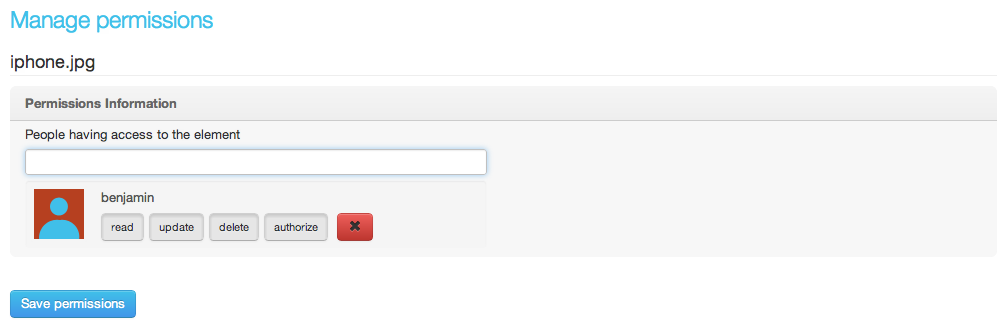
\includegraphics[width=0.97\textwidth]{images/set-model-permissions.png}
  }
  \caption{Set permissions on an entity}
  \label{fig:set-model-permissions}
\end{figure}

The permission check on models does have to be done by hand in any controller action, where needed. A simple selection of the required permission and then a call of the hasPermission-method on the user role is sufficient. The following example checks the users read permission on a specific document:

\begin{lstlisting}[caption=Checking the user permission on an entity]
$permission = $this->_em->getRepository('Application_Model_ModelPermission')->findOneBy(array('type'=>'document', 'action'=>'read', 'base'=>$document));
if(Zend_Registry::getInstance()->user->getRole()->hasPermission($permission)){
	// user has access
}
\end{lstlisting}

\textbf{Page permissions}

The second type of permissions are the page permissions. They control access to controller and action methods. This means, they define whether a user can for example access the page /document/list or not. The available permissions are being generated on each deployment of the site automatically. So when a new action in a controller is created, it will be available as a new permission after the next deployment.


\section{Barcode}
The barcode is a visual representation of the amount of plagairism in each page of the target document. In our application it is used in two representations, which use the same data source but have another visual layout and details shown within.

The barcode has 4 different colors, which represent another amount of plagairism within the page:

\begin{itemize}
\item      light blue: the page is disabled for the barcode
\item      white: page not available or no plagiarism
\item      black: more than 0 percent plagiarized
\item      dark red: more than percent plagairized
\item      light red: more than percent plagairized
\end{itemize}

\textbf{Representation with labels on the home page}

The first representation can be found at the home page, here are the barcodes of all published cases being displayed. The barcode is being displayed with page numbers below and the width is dynamic, so the barcode increases when the page gets wider and the barcode gets smaller, when the page width decreases. 

\begin{figure}[!h]
  \centering
  \fbox{
    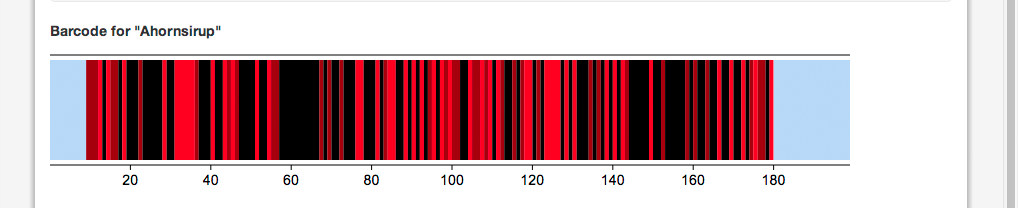
\includegraphics[width=0.97\textwidth]{images/feature-barcode-website.png}
  }
  \caption{Barcode on home page}
  \label{fig:feature-barcode-website}
\end{figure}

Since this mechanism is very dynamic, an algorithm needed to be developed to calculate the x axis values taking into consideration the page width and the number of pages in the document being visualized. It assumes that a label needs at least 45px of width and the whole barcode has to look well to a width of 500px.

So what we do is, we start with a setpsize of 10 for the page numbers: 10 20 30 40 50, now we check if the amount of pages can be displayed with such a fine scale to stay in the 500px range. For example a page count of 200 leeds to 20 values on the x axis and if we assume 45px are necessary to display a value on the axis properly, we would need 900px of width, but we have only 500px available. Otherwise we would have crossovers when we get below 900px. So the stepsize is increased by 10, until we stay in the 500px maximum width. As it turns out, a step size of 20 pages is sufficent to get a width of 450px in the end. The code for this calculation is being shown below.

\begin{lstlisting}[caption=Generating the barcode x axis]
private function generateAxis() {
        $labelStepsize = 10;

        while (true) {
            $count = sizeof($this->pages);
            $labelCount = floor($count / $labelStepsize);

            // we assume a label needs 45px and 500px is the width that needs to be displayable without crossovers
            if (45 * $labelCount > 500) {
                $labelStepsize += 10;
                continue;
            }
            break;
        }

        $label = $labelStepsize;
        $x = 0;
        while ($x < ($this->width - ($this->initWidth * $labelStepsize))) {
            $x += ($this->initWidth * $labelStepsize);
            $this->result .= '<text x="' . $x . $this->widthUnit . '" y="' . $this->y . '" font-family="Arial" font-size="14" text-anchor="middle">' . $label . '</text>';
            $this->result .= '<line x1="' . $x . $this->widthUnit . '" y1="' . ($this->y - 20) . '" x2="' . $x . $this->widthUnit . '" y2="' . ($this->y - 15) . '" stroke-width="1" stroke="#000000"></line>';

            $label += $labelStepsize;
        }
    }
\end{lstlisting}

\textbf{Representation without labels in the report}

The second area where barcodes are used, are the final reports. They will be explained in the next section. The space available in the PDF is much less than on the website and the library we are using for generating the PDF report does not support text in scable vectors graphics, so we decided to display the barcodes without labels for now. However the data visualized is exactly the same.

\section{Report}

The report is needed to collect and document all the found plagiarized fragments of the reviewed document. It will be used as an evidence proof.
The report documents all founded plagiarized parts including the corresponding sources.

The report has also a barcode on the first page to give the reader a quick visuell overview to the plagiarization level of the reviewed document.

Below you can see the generation and the outlook of an example of a report.

\subsection{Generating of a Report}

To generate a report it is neccessary that there exist approved fragments for this case. Without approved fragments in a case it is not possible to generate a report for this case. 
This is made to have only approved fragments listed in the report. This makes sure that only real plagiarized textparts are listed in the report.

To generate a report the user needs to choose the tab `Berichte' and than click at the button `Bericht erstellen'. After the user clicked at the  button `Bericht erstellen' it has the possibility to fill up the report form to give the title of the report and to give some evaluations about the reviewed document.

After the user saved the entries of the form the report will be generated and the report will be listed.

\subsection{Outlook of a Report}

The report has three different parts. The evaluation text, the list of approved fragments and the references to the sources.
